\documentclass[a4paper,12pt]{article}

\usepackage[utf8]{inputenc}
\usepackage[T1]{fontenc}
\usepackage[spanish]{babel}
\usepackage{caption}
\usepackage{amsfonts, amsmath, amssymb, enumitem, authblk, times, framed, varwidth, graphicx, placeins, indentfirst, pdfpages, fancyhdr, titling, listings} 
\usepackage{float}
\usepackage[justification=centering]{caption}
\setlength{\textwidth}{180mm}
\setlength{\textheight}{250mm}
\setlength{\oddsidemargin}{-10mm}
\setlength{\evensidemargin}{15mm}
\setlength{\topmargin}{-10mm}

\renewcommand{\baselinestretch}{1.4}
\renewcommand{\headrulewidth}{0.5pt}

\lhead{\begin{picture}(0,0) \put(0,0){
\includegraphics[width=20mm]{./LogoITBA}} \end{picture}}
\renewcommand{\headrulewidth}{0.5pt}

\def\FIG#1#2{%
	{\centering#1\par}
	#2}

\pagestyle{fancy}

\begin{document}
	
	\begin{titlepage}
		\centering
		{
\includegraphics[width=0.50\textwidth]{LogoITBA}\par}
		{\bfseries\LARGE Instituto Tecnol\'ogico de Buenos Aires \par}
		\vspace{2cm}
		{\scshape\Huge StegoBMP \par}
		\vspace{1cm}
		{\itshape\Large 72.44 Criptografía y Seguridad - 2024Q1 \par}
		\vspace{3cm}
		{\Large Tom\'as Marengo - 61587 \par}
		{\Large tmarengo@itba.edu.ar \par}	
		\vfill
	\end{titlepage}
	
	\newpage
	\tableofcontents
	\newpage
	
	\section{Introducción}
	La esteganografía es la práctica de ocultar información dentro de otro objeto, de manera que su existencia no sea perceptible a simple vista. A lo largo de la historia, se han utilizado diversas técnicas esteganográficas para proteger la confidencialidad de la información. En el contexto digital, una de las técnicas más comunes consiste en ocultar datos en archivos de imagen modificando sus bits menos significativos (LSB, por sus siglas en inglés).
	
	Este trabajo práctico tiene como objetivo implementar y probar un sistema de esteganografía digital utilizando diferentes métodos de inserción en los bits menos significativos de imágenes BMP. Además, se exploran técnicas de cifrado para proteger la información antes de ocultarla, garantizando así una capa adicional de seguridad. El objetivo es garantizar que la información sea indetectable y, en caso de ser descubierta, inaccesible sin la clave adecuada.

	\section{Diseño del sistema}
	
	El sistema está diseñado en una arquitectura modular que consta de las siguientes partes:
	
	\begin{itemize}
		\item \textbf{Operator:} Clase base que contiene los parámetros comunes a las operaciones de ocultamiento y extracción.
		\item \textbf{Embedder:} Clase derivada de Operator, responsable del ocultamiento de datos en una imagen BMP.
		\item \textbf{Extractor:} Clase derivada de Operator, responsable de la extracción de datos de una imagen BMP.
		\item \textbf{SteganographyUtil:} Contiene métodos estáticos para la encriptación y desencriptación de datos, así como constantes utilizadas en todo el sistema.
		\item \textbf{Steganography:} Punto de entrada del programa que parsea los argumentos de la línea de comandos y coordina las operaciones de ocultamiento y extracción.
	\end{itemize}

	\newpage

	\section{Stegoanálisis de los archivos provistos}
	
	\begin{itemize}

		\item \textit{Explicar detalladamente el procedimiento realizado para descubrir qué se había ocultado en cada archivo y de qué modo. Indicar qué se encontró en cada archivo.}
	
		Por enunciado se sabe que por lo menos hay un archivo esteganografiado por cada método, por lo que primero probé extraer cada archivo con cada método (LSB1, LSB4, LSBI). Dos de ellos no generaron errores de ejecución, porque estaban simplemente esteganografiados sin cifrado:
		
		\framebox[10.3cm][c]{-extract -p mystery/kings.bmp -out extracted/ -steg LSB1}
		
		\framebox[10.3cm][c]{-extract -p mystery/paris.bmp -out extracted/ -steg LSBI}
		
		Esos dos generaron, respectivamente, un archivo .png de un buscaminas y un .pdf con una password (\textit{sorpresa}) a utilizar. El PDF entonces me dijo que uno de los archivos restantes estaba cifrado (y por eso me generaba errores de ejecución). Lo que quedaba descubrir era el algoritmo y modo de cifrado utilizado. 
		
		También se sabe por enunciado que uno de los archivos restantes tenía información pertinente, pero no esteganografiada. Lo primero que se me ocurrió fue analizar los archivos restantes con un editor hexadecimal (HxD) y descubrí que \textit{loimposible.bmp} tenía al final de todo, la frase: \textit{``al .png cambiar extension por .zip y descomprimir''}.
		
		Ya tenía un archivo .png, el archivo del buscaminas, por lo que le cambié la extensión. Al descomprimirlo, me encontré con unas instrucciones dentro de un .txt que debía aplicar sobre el buscaminas. Haciendo el puzzle obtuve en formato binario:
		
		\begin{center}
				\begin{varwidth}{\linewidth}
					\begin{verbatim}
						01000001
						01100101
						01110011
						01000011
						01100010
						01100011
					\end{verbatim}
				\end{varwidth}
		\end{center}
	
		Es decir, ``AesCbc''.
		
		Me quedaba probar entonces la longitud de key usada para AES (128, 196 o 256). Finalmente con:
		
		\framebox[16.3cm][c]{-extract -p mystery/lima.bmp -out extracted/ -steg LSB4 -a AES128 -m cbc -pass sorpresa}
		
		obtuve un archivo .wmv con una parte de una película, un diálogo entre dos personajes (ver más abajo).
		
		\newpage
		
		\item \textit{Algunos mensajes ocultos tenían, a su vez, otros mensajes ocultos. Indica cuál era ese mensaje y cómo se había ocultado.}

		Mencionado arriba. La imagen del buscaminas al cambiarle la extensión a zip, ocultaba otra información (las instrucciones para analizar el buscaminas).

		\item \textit{Uno de los archivos ocultos era una porción de un video de una película, donde se ve ejemplificado una manera de ocultar información. ¿Qué se ocultaba y sobre qué portador?}

		Los métodos de esteganografía que vimos usan los mismos bytes de un archivo para ocultar información. En el video, por otra parte, nombra que se usó un método que alargó la longitud del archivo. Investigando un poco, este podría ser un método de inserción de bits, de expansión de texto, de codificación Run-Length, etc.
		
		\item \textit{¿De qué se trató el método de esteganografiado que no era LSB1 ni LSB4 ni LSBI? ¿Es un método eficaz? ¿Por qué?}
		
		Se cambiaron los últimos bytes del archivo \textit{loimposible.bmp} para incluir un texto plano con instrucciones a seguir (\textit{``al .png cambiar extension por .zip y descomprimir''}). Claramente no es un método eficaz porque con cualquier editor hexadecimal vas a poder extraer esa información fácilmente, más aún si está en ubicaciones fáciles de encontrar (como el final) o si el archivo no es tan pesado (es decir, que no requiera tanto análisis para encontrar textos con sentido). Además analizar la imagen con el editor es una de las primeras cosas que se te ocurren.
	
	\end{itemize}
	
	\newpage
	
	\section{Cuestiones a Analizar}
	
	\begin{itemize}
		\item \textit{Discutir los siguientes aspectos relativos al documento.}
		\begin{itemize}
			\item \textit{a) Organización formal del documento:}
			
			Contiene por lo menos parte de la estructura típica de un paper: encabezamiento del informe, título, autoría, resumen (abstract), instroducción, discusión y conclusión, y referencias; en el medio de esto, todo el detalle del método. 
			
			\item \textit{b) La descripción del algoritmo:}
			
			Propone un ejemplo y el pseudocódigo no es complejo, por lo que no es complicado de leer.

			
			\item \textit{c) La notación utilizada, ¿es clara? ¿hay algún error o contradicción?}
			
			Es claro, pero con algunos errores gramaticales. Además, yo agregaría casos relacionados a la extracción y no sólo al ocultamiento, ya que quedan preguntas sin responder, por ejemplo cuál es la mejor forma de guardar los patrones. 

		\end{itemize}
		
		\item \textit{Esteganografiar un mismo archivo en un .bmp con cada uno de los tres algoritmos, y comparar los resultados obtenidos. Hacer un cuadro comparativo de los tres algoritmos estableciendo ventajas y desventajas.}
			
		\begin{figure}[h!]%
			\FIG{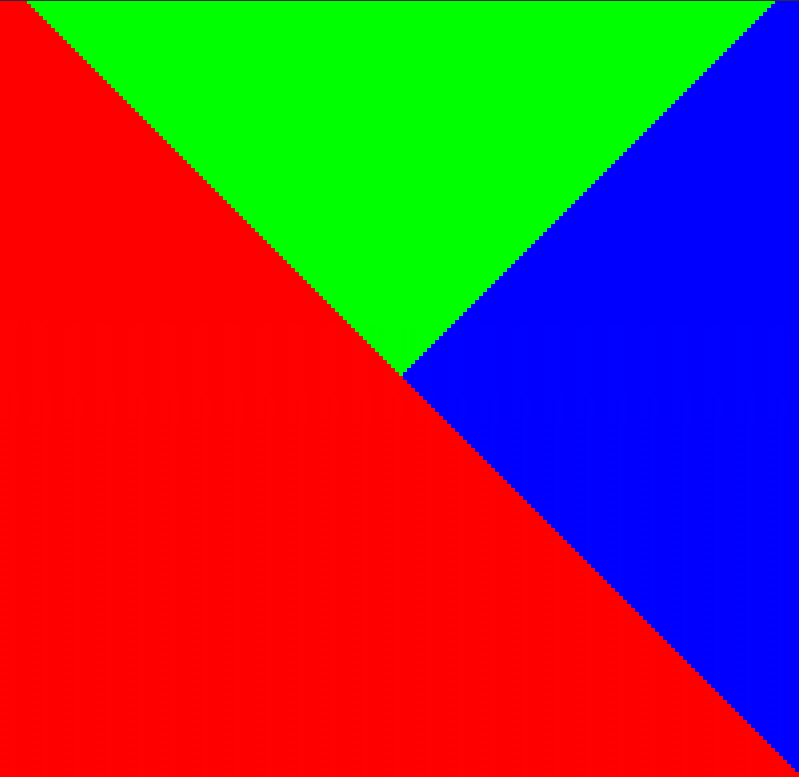
\includegraphics[width=0.5\textwidth]{tricolor_lsb1.png}}
			{\caption{Imagen con un mensaje oculto con LSB1.}
				\label{fig1}}
		\end{figure}
	
		\newpage
		
		\begin{figure}[h!]%
			\FIG{
\includegraphics[width=0.5\textwidth]{tricolor_lsb4.png}}
			{\caption{Imagen con un mensaje oculto con LSB4.}
				\label{fig2}}
		\end{figure}
	
		\begin{figure}[h!]%
			\FIG{
\includegraphics[width=0.5\textwidth]{tricolor_lsbi.png}}
			{\caption{Imagen con un mensaje oculto con LSBI.}
				\label{fig3}}
		\end{figure}
	
	
		En LSB4 se puede notar claramente en la parte de abajo cómo cambió el color rojo. En LSB1 hay que forzar mucho la vista para poder notar un cambio en este color. Finalmente, en LSBI no se nota nada (en este caso particular donde al principio son todos píxeles rojos).
		
		\begin{table}[H]
			\centering
			\begin{tabular}{|c|p{7cm}|p{7cm}|}
				\hline
				\textbf{Método} & \textbf{Ventajas} & \textbf{Desventajas} \\
				\hline
				\textbf{LSB1} & 
				\begin{itemize}
					\item Fácil de implementar
					\item Baja distorsión visual
					\item Alta capacidad de almacenamiento
				\end{itemize} &
				\begin{itemize}
					\item Baja robustez contra ataques de compresión y manipulación de imagen
					\item Fácil de detectar con análisis estadístico
				\end{itemize} \\
				\hline
				\textbf{LSB4} & 
				\begin{itemize}
					\item Mayor capacidad de almacenamiento que LSB1
					
				\end{itemize} &
				\begin{itemize}
					\item Moderada distorsión visual
					\item Baja robustez contra ataques de compresión y manipulación de imagen
				\end{itemize} \\
				\hline
				\textbf{LSBI} & 
				\begin{itemize}
					\item Mayor robustez contra ataques
					\item Buena calidad de imagen
					\item Balance entre capacidad y seguridad
				\end{itemize} &
				\begin{itemize}
					\item Más complejo de implementar
					\item Menor capacidad de almacenamiento comparado con LSB4
				\end{itemize} \\
				\hline
			\end{tabular}
			\caption{Comparación de métodos de esteganografía: LSB1, LSB4 y LSBI}
			\label{tab:comparison}
		\end{table}
		
		
		\item \textit{¿Por qué la propuesta del documento de Majeed y Sulaiman es realmente una mejora respecto de LSB común?}
		
		Porque añade varias capas de seguridad: al invertir los bits de ciertos píxeles en la imagen, después de aplicar LSB1, se dificulta la recuperación de mensajes secretos por parte de un atacante ya que primero debería deducir el patrón utilizado para invertir o saber de dónde recuperarlo. Además al no usar los pixéles rojo, estos actúan como datos de ruido, aumentando la complejidad del proceso de extracción. También busca minimizar la cantidad de píxeles modificados en comparación con los métodos LSB1 y LSB4. Esto conduce a una mejora en la calidad de la imagen esteganográfica resultante. También se puede ver por definición de entropía, la incertidumbre es más alta ya que la información es menor, esto se debe a que hay menos píxeles modificados, por lo que la distribución se acercaría más a la de una imagen real.
		
		\newpage 
		
		\item \textit{En la implementación se optó por guardar los patrones invertidos al final del mensaje. ¿Es esta una opción más segura que guardarlos antes del mensaje? ¿Por qué?}
		
		Si se guardara al principio, saber dónde están los patrones sería trivial ya que siempre se sabe el principio, pero al guardarlo en el final, no es tan trivial saber dónde empieza ese final. Sin embargo, esto último necesita de algún dato que nos diga dónde comienzan los patrones en ese final. Pero eso genera un nuevo problema, porque si se sabe dónde está ese dato, por diseño abierto, entonces también se vuelve trivial saber dónde comienza el final.
		
		En el caso de LSBI existía un problema en el enunciado, que luego planteé. Nosotros sabíamos que los patrones estaban luego de la extensión (string null terminated), pero nunca podríamos saber dónde terminaba la extensión (o sería muy difícil de determinar) ya que el carácter nulo también podría estar invertido.
		
		\item \textit{¿De qué otra manera o en qué otro lugar podría guardarse el registro de los patrones invertidos?}
		
		Como mencioné, se podría agregar al principio o al final. Además, se podría guardar en cualquier otro lado, pero deberíamos tener otro dato para saber dónde (por ejemplo si decidieramos incluirlo en la mitad, tendríamos que saber dónde está la mitad efectivamente). Caemos nuevamente en tener que ocultar otro dato (en nuestro ejemplo, la ubicación de la mitad) para saber donde está otro dato (nuestros patrones). Esto dificultaría un poco el análisis que tenga que hacer el atacante, pero cualquiera que sepa cómo funciona nuestro algoritmo, sabrá donde están esos datos.
		
		Analizando temas vistos en la materia, otra forma podría ser trasmitirlos por un canal seguro y no dentro de la imagen. De esta forma los patrones sólo lo sabrían las dos partes y no un atacante. Sin embargo, si los patrones son sólo 4 bits, el atacante solo debería intentar 16 formas, por lo que se podría hacer en un tiempo razonable por fuerza bruta. No lo veo tan seguro cualquiera sea la forma.
		
		\item \textit{¿Qué dificultades encontraron en la implementación del algoritmo del paper?}
		
		Sin duda el manejo de bits y bytes, que siempre es un dolor de cabeza (operaciones de shifteo, and y or a nivel bit, etc.)
		
		\item \textit{¿Qué mejoras o futuras extensiones harías al programa stegobmp?}
		
		Un análisis testeando los diferentes algoritmos (y agregando otros que encuentre publicados por la comunidad). La idea sería sacar conclusiones matemáticas de cuáles sirven más y en qué casos. Pueden haber imágenes con colores de píxeles particulares donde un algoritmo sirva más que otro, por ejemplo, en LSBI al no tocar píxeles rojos, cualquier imagen con tonalidades rojizas, escondería fácilmente mensajes ocultos.
		
		Aprovechando la clase de flujo de información, otra de las mejoras sería un análisis de entropía para cada método. Antes de enviar una imagen esteganografiada, se pasaría por diferentes métodos y se enviaría aquel que tenga la mayor entropía. También se podría comprimir/cifrar para mejorar la entropía (ya que se acercaría más a valores aleatorios).
	
	\end{itemize}
	

\end{document}
